% ============================================================
% §3 Implementation — C 主笔 · 页数预算 1.5 · 素材 C1/C3/C4/C5
% SQL 关（11-02）检查项：干净环境从零复跑 build.sql + 导数成功
% 2026-11-04 成稿（数字经真机验收：seed=534，Payment=51,398）
% ============================================================
\section{Implementation}
\label{sec:impl}

The design of Section~\ref{sec:er} is realised by three repository artefacts: the idempotent build
script \texttt{02\_sql/build.sql} (\S\ref{sec:ddl}), the deterministic data generator
\texttt{02\_sql/import\_data.py} (\S\ref{sec:data}), and a clean-room acceptance procedure with a
standardised screenshot package (\S\ref{sec:verify}).

\subsection{Environment and Architecture}
\label{sec:env}
All five members work on a local MySQL~8 instance under one shared schema, \texttt{ride\_hailing}
(\texttt{utf8mb4\_general\_ci}); the group compatibility baseline is the lowest registered server
version (8.0.45), so the scripts avoid CTEs and window functions and treat pre-8.0.16 servers as
silently ignoring CHECK constraints. GitHub is the single source of truth: a schema change counts
only when it lands in \texttt{build.sql} (``change the table = change the script = commit''), and
after every pull members rebuild the database from scratch, keeping the five environments identical
by construction. Screenshot evidence follows a written specification (naming
\texttt{prefix\_object\_MMDD.png}; whole-window captures keeping the statement, the result grid and
the action-output panel in one frame), so every figure in this report traces back to the exact
machine, script and statement that produced it.

\subsection{DDL Organisation and Key Constraints}
\label{sec:ddl}
\texttt{build.sql} is organised in four blocks: (0)~drop/recreate the schema; (1)~the official
five-table DDL of Topic~5, kept unmodified in the repository (``base immutability rule'');
(2)~the official seed queries; (3)~the extension zone; (4)~a self-check block printing the server
version, the table list and per-table counts, turning every rebuild into a verifiable event.
Extensions never touch the five base tables: two seeded dimension tables (\texttt{service\_tier},
four tiers calibrated to RideAustin shares; \texttt{pickup\_zone}, 15 zones) and one 1:1 extension
table \texttt{trip\_detail} whose primary key is also a foreign key to \texttt{Trip}.
Table~\ref{tab:constraints} maps each ER cardinality to the constraint that enforces it.

\begin{table}[ht]
\centering
\caption{ER cardinalities and their SQL enforcement (\texttt{build.sql}).}
\label{tab:constraints}
\begin{tabular}{@{}lll@{}}
\toprule
Relationship & Constraint & Cardinality \\
\midrule
Trip--Payment & \texttt{Payment.trip\_id NOT NULL UNIQUE} + FK & 1:(0..1) \\
Vehicle--Driver & \texttt{Driver.vehicle\_id NOT NULL UNIQUE} + FK & 1:(0..1) \\
Passenger/Driver--Trip & NOT NULL FKs & 1:N mandatory \\
ServiceTier/PickupZone--TripDetail & NOT NULL FKs & 1:N mandatory \\
Trip--TripDetail & \texttt{trip\_id} PK-as-FK & 1:(0..1) \\
\bottomrule
\end{tabular}
\end{table}

One design rule cannot be expressed in DDL: \texttt{rating} must be non-NULL only for completed
trips --- a cross-table condition that CHECK cannot reference. It is enforced by the generator and
documented as a deliberate constraint-expressiveness boundary; trigger-based enforcement was
considered out of course scope.

\subsection{Data Generation and Import}
\label{sec:data}
The generator uses the Python standard library only --- no third-party dependencies --- so all five
machines produce identical output regardless of installed packages. A single seeded RNG
(\texttt{seed=534}) drives exact-composition pools: each categorical attribute (status, payment
method, tier mix, rating) is drawn from a pool with exact counts and then shuffled, so proportions
are exact and only the order is random. Fares follow the group's RideAustin-calibrated formula ---
base + per-minute + per-mile + a fixed \$1.65 surcharge; the REGULAR tier uses a two-period mile
tariff (0.99/1.50 per mile, 80/20 split) --- and free cancellation (no payment row), charged
cancellation (\$1.50) and completed-but-unpaid trips are all represented per the fare-calibre
decision. Determinism was verified by generating the import file twice and comparing checksums: the
174{,}698-statement \texttt{data\_import.sql} is byte-identical across runs and machines.
Table~\ref{tab:rows} lists the resulting row counts.

\begin{table}[ht]
\centering
\caption{Row counts after a clean rebuild and import (\texttt{seed=534}).}
\label{tab:rows}
\begin{tabular}{@{}lcccccccc@{}}
\toprule
 & Passenger & Vehicle & Driver & Trip & Payment & service\_tier & pickup\_zone & trip\_detail \\
\midrule
Rows & 3{,}000 & 150 & 150 & 60{,}000 & 51{,}398 & 4 & 15 & 60{,}000 \\
\bottomrule
\end{tabular}
\end{table}

\subsection{Verification}
\label{sec:verify}
Acceptance was defined as a clean-room procedure: drop the schema, run \texttt{build.sql}, import
\texttt{data\_import.sql}, then execute the twelve-statement acceptance script
\texttt{02\_sql/c5\_check.sql}. It re-derives the eight table counts of Table~\ref{tab:rows}, runs
zero-anomaly checks (no orphaned foreign keys, no trip without an extension row, no payment for a
non-existent trip), and spot-checks business queries against pre-computed expected values: the first
Q1 row (trip~1, Justin Lewis, fare 8.33, cash), exactly 150 drivers with completed-unpaid trips
(Q2), and the four-tier aggregate of q10. Every check passed with observed values identical to
expected. Evidence is captured per the screenshot specification: 21 verification screenshots
(2026-11-01) --- structure and row count for each of the eight tables, the row-count summary
(Fig.~\ref{fig:rowcounts}), and four query spot-checks --- plus the ten query-result screenshots
referenced in Section~\ref{sec:sql}. The procedure simultaneously closes goal G1
(60{,}000 trips $\geq$ 50{,}000) and demonstrates goal G5 (constraint enforcement; error-code
demonstrations appear with the experiments in Section~\ref{sec:eval}).

\begin{figure}[ht]
\centering
\begin{minipage}{0.48\textwidth}\centering
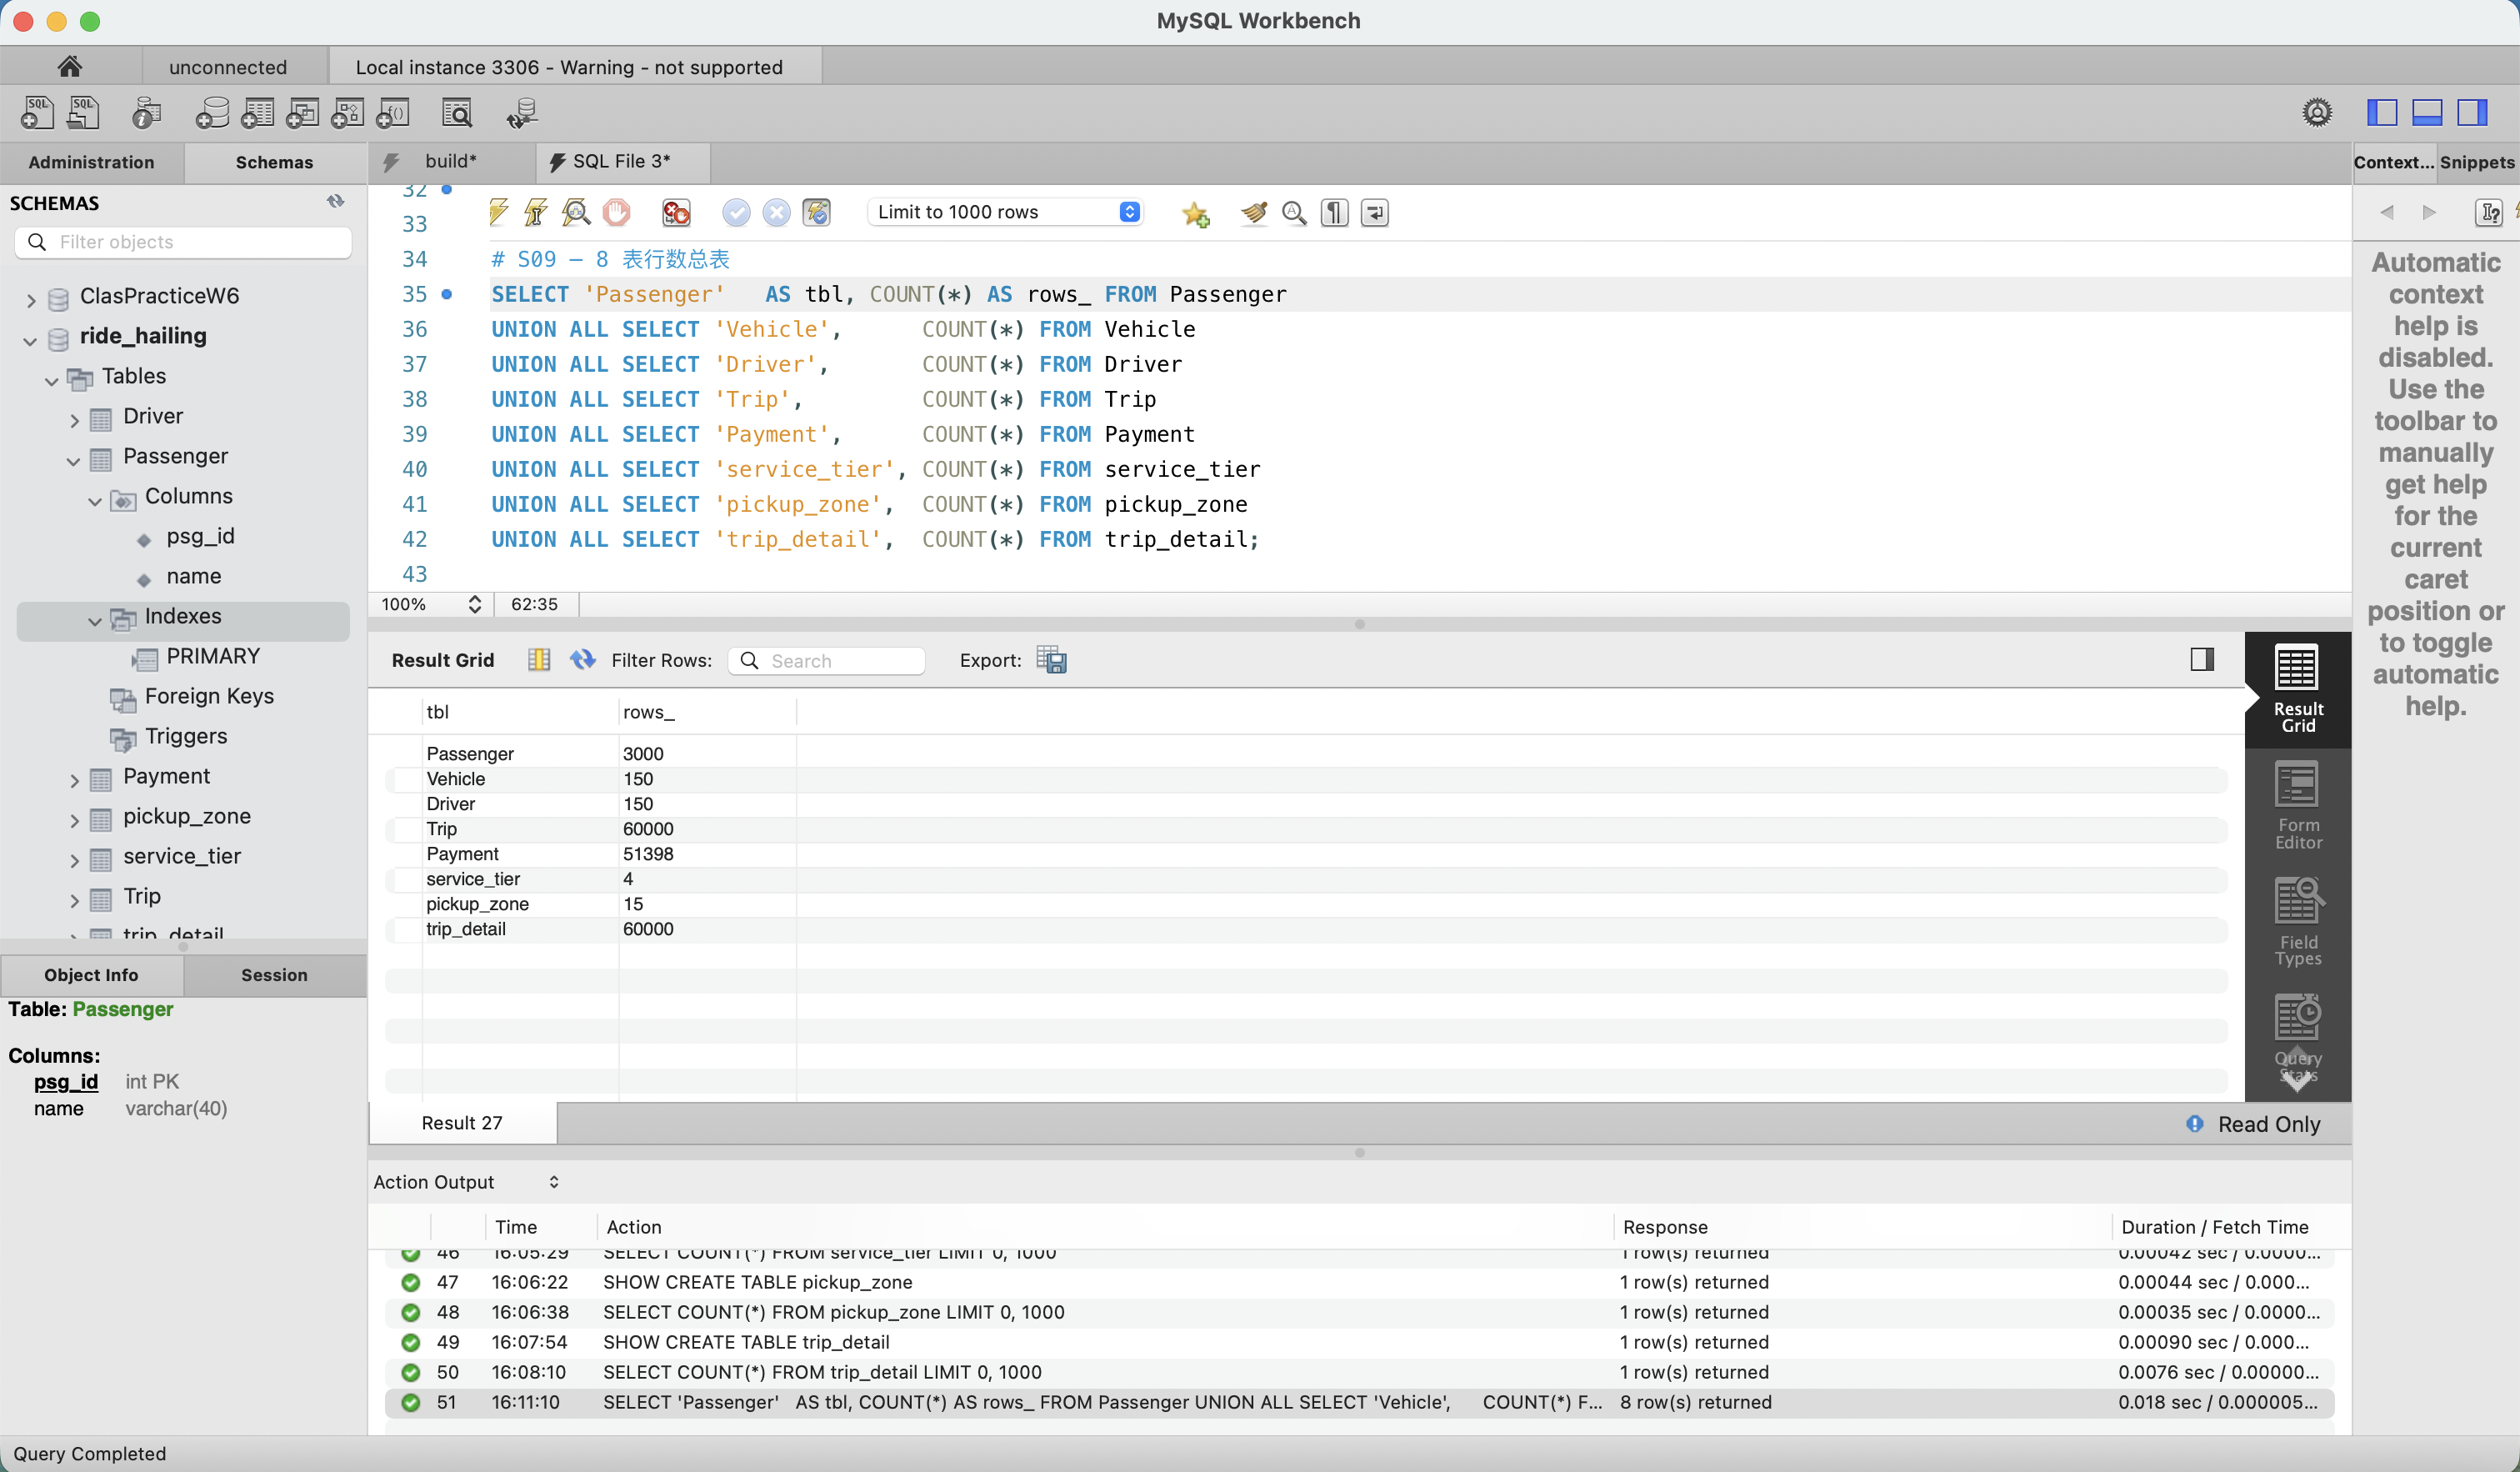
\includegraphics[width=\linewidth]{row_counts_1101.png}
\caption{Eight-table row-count self-check.}\label{fig:rowcounts}
\end{minipage}\hfill
\begin{minipage}{0.48\textwidth}\centering
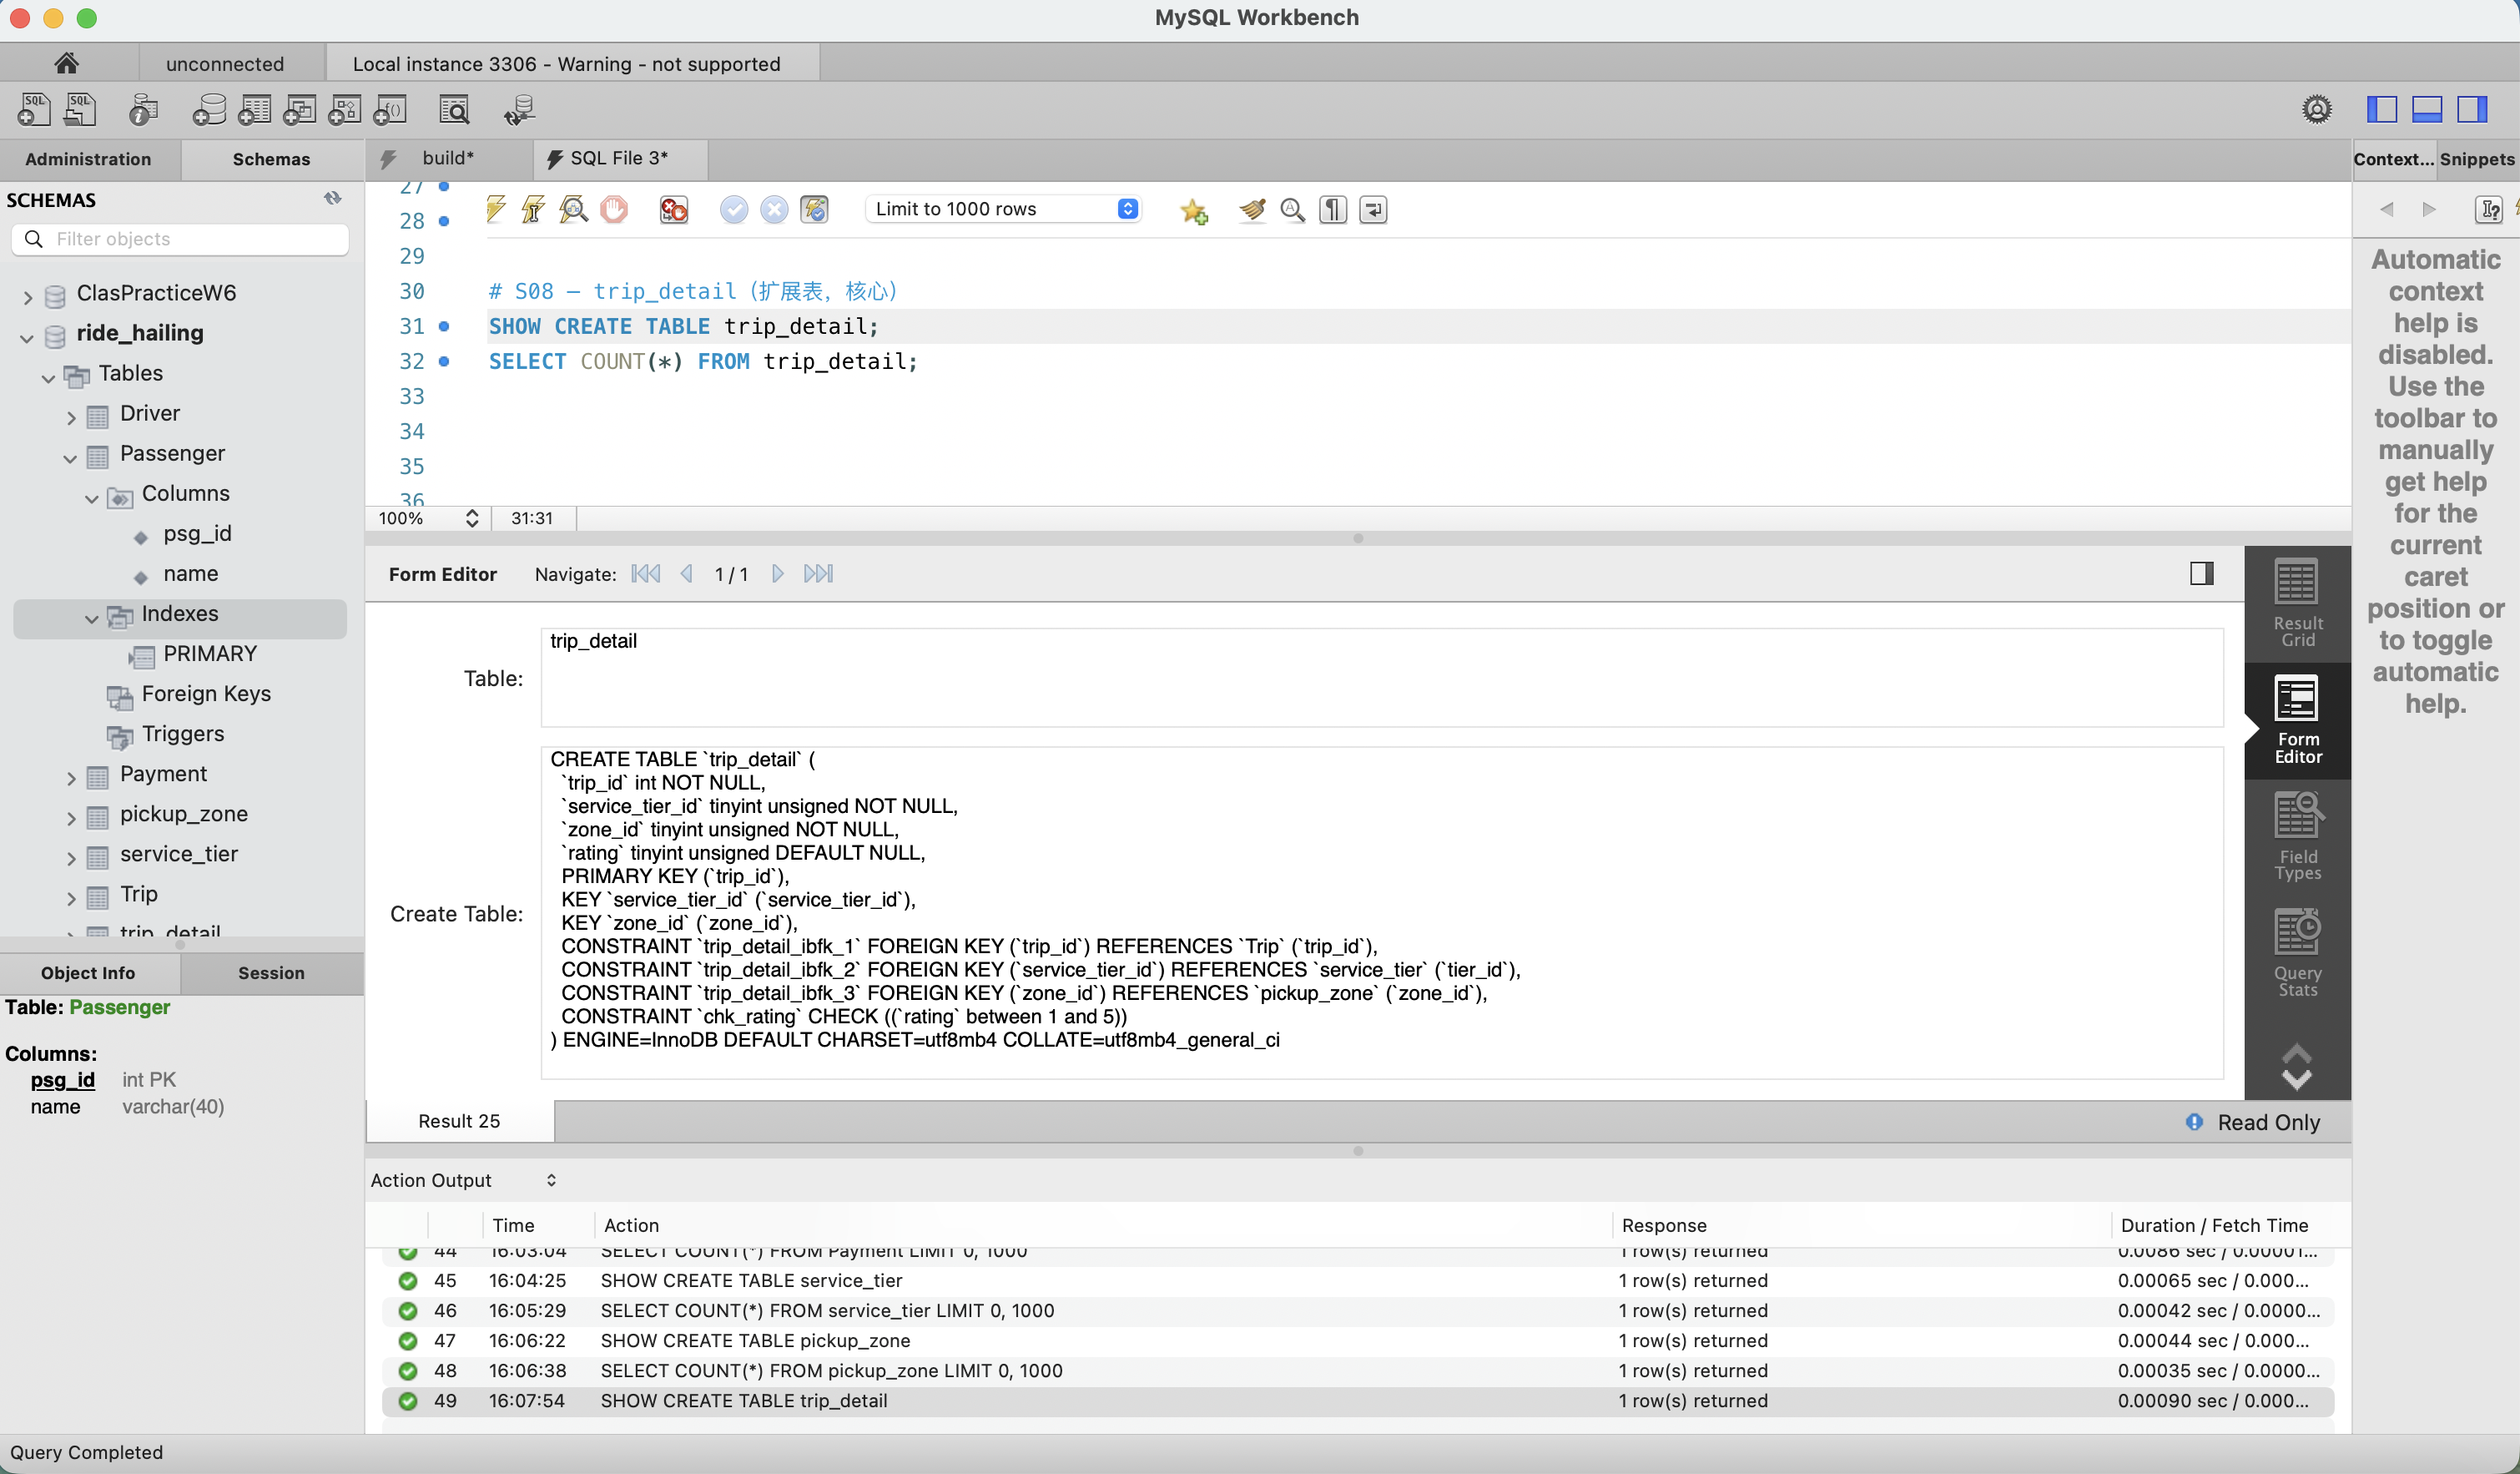
\includegraphics[width=\linewidth]{ddl_trip_detail_1101_a.png}
\caption{\texttt{trip\_detail} DDL: PK-as-FK, three FKs, rating CHECK.}\label{fig:tripdetail}
\end{minipage}
\end{figure}
